\section{Date: 2026-09-16}
\noindent \textbf{Series ID: EMISSCO2VDFCCBA} 

\noindent This series is titled Distillate Fuel Commercial Sector Carbon Dioxide Emissions and has a frequency of Annual. The units are Million Metric Tons CO2 and the seasonal adjustment is Not Seasonally Adjusted.The observation start date is 1973-01-01 and the observation end date is 2024-01-01.The popularity of this series is 1. \\ 

\noindent \textbf{Series ID: BRVSLV02JPQ460S} 

\noindent This series is titled Business Tendency Surveys: Volume of Stocks: Economic Activity: Retail Trade, Except of Motor Vehicles and Motorcycles: Current for Japan and has a frequency of Quarterly. The units are Percentage balance and the seasonal adjustment is Seasonally Adjusted.The observation start date is 1990-10-01 and the observation end date is 2026-04-01.The popularity of this series is 1. \\ 

\subsection{Raw Regression}
\noindent Regresses the two series against each other directly. A significant result here can come just as easily from both series sharing a long-run trend as from any real relationship.

\begin{center}
\begin{tabular}{lclc}
\toprule
\textbf{Dep. Variable:}               & value\_fred\_BRVSLV02JPQ460S & \textbf{  R-squared:         } &     0.481   \\
\textbf{Model:}                       &             OLS              & \textbf{  Adj. R-squared:    } &     0.465   \\
\textbf{Method:}                      &        Least Squares         & \textbf{  F-statistic:       } &     29.65   \\
\textbf{Date:}                        &       Wed, 16 Sep 2026       & \textbf{  Prob (F-statistic):} &  5.44e-06   \\
\textbf{Time:}                        &           15:39:06           & \textbf{  Log-Likelihood:    } &   -112.36   \\
\textbf{No. Observations:}            &                34            & \textbf{  AIC:               } &     228.7   \\
\textbf{Df Residuals:}                &                32            & \textbf{  BIC:               } &     231.8   \\
\textbf{Df Model:}                    &                 1            & \textbf{                     } &             \\
\textbf{Covariance Type:}             &          nonrobust           & \textbf{                     } &             \\
\bottomrule
\end{tabular}
\begin{tabular}{lcccccc}
                                      & \textbf{coef} & \textbf{std err} & \textbf{t} & \textbf{P$> |$t$|$} & \textbf{[0.025} & \textbf{0.975]}  \\
\midrule
\textbf{const}                        &     -20.4615  &        6.786     &    -3.015  &         0.005        &      -34.285    &       -6.638     \\
\textbf{value\_fred\_EMISSCO2VDFCCBA} &       1.2106  &        0.222     &     5.445  &         0.000        &        0.758    &        1.664     \\
\bottomrule
\end{tabular}
\begin{tabular}{lclc}
\textbf{Omnibus:}       &  6.618 & \textbf{  Durbin-Watson:     } &    1.027  \\
\textbf{Prob(Omnibus):} &  0.037 & \textbf{  Jarque-Bera (JB):  } &    5.041  \\
\textbf{Skew:}          & -0.838 & \textbf{  Prob(JB):          } &   0.0804  \\
\textbf{Kurtosis:}      &  3.867 & \textbf{  Cond. No.          } &     178.  \\
\bottomrule
\end{tabular}
%\caption{OLS Regression Results}
\end{center}

Notes: \newline
 [1] Standard Errors assume that the covariance matrix of the errors is correctly specified.

\begin{figure}
\centering
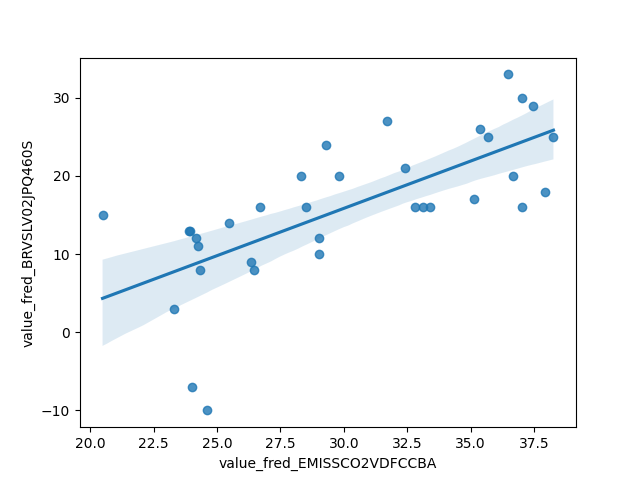
\includegraphics[scale = 0.9]{plots/plot_2026-09-16.png}
\caption{Raw Regression Plot for 2026-09-16}
\end{figure}
\newpage
\subsection{Detrended Regression}
\noindent Regresses the residuals of each series after removing its own linear time trend, so a shared trend can no longer drive the result on its own. A relationship that stays significant here is better evidence of a genuine link between the two series.

\begin{center}
\begin{tabular}{lclc}
\toprule
\textbf{Dep. Variable:}                          & value\_fred\_BRVSLV02JPQ460S\_detrended & \textbf{  R-squared:         } &     0.166   \\
\textbf{Model:}                                  &                   OLS                   & \textbf{  Adj. R-squared:    } &     0.140   \\
\textbf{Method:}                                 &              Least Squares              & \textbf{  F-statistic:       } &     6.379   \\
\textbf{Date:}                                   &             Wed, 16 Sep 2026            & \textbf{  Prob (F-statistic):} &   0.0167    \\
\textbf{Time:}                                   &                 15:39:06                & \textbf{  Log-Likelihood:    } &   -100.08   \\
\textbf{No. Observations:}                       &                      34                 & \textbf{  AIC:               } &     204.2   \\
\textbf{Df Residuals:}                           &                      32                 & \textbf{  BIC:               } &     207.2   \\
\textbf{Df Model:}                               &                       1                 & \textbf{                     } &             \\
\textbf{Covariance Type:}                        &                nonrobust                & \textbf{                     } &             \\
\bottomrule
\end{tabular}
\begin{tabular}{lcccccc}
                                                 & \textbf{coef} & \textbf{std err} & \textbf{t} & \textbf{P$> |$t$|$} & \textbf{[0.025} & \textbf{0.975]}  \\
\midrule
\textbf{const}                                   &   -6.513e-13  &        0.812     & -8.02e-13  &         1.000        &       -1.654    &        1.654     \\
\textbf{value\_fred\_EMISSCO2VDFCCBA\_detrended} &      -1.0600  &        0.420     &    -2.526  &         0.017        &       -1.915    &       -0.205     \\
\bottomrule
\end{tabular}
\begin{tabular}{lclc}
\textbf{Omnibus:}       &  7.112 & \textbf{  Durbin-Watson:     } &    1.687  \\
\textbf{Prob(Omnibus):} &  0.029 & \textbf{  Jarque-Bera (JB):  } &    5.544  \\
\textbf{Skew:}          & -0.868 & \textbf{  Prob(JB):          } &   0.0625  \\
\textbf{Kurtosis:}      &  3.947 & \textbf{  Cond. No.          } &     1.93  \\
\bottomrule
\end{tabular}
%\caption{OLS Regression Results}
\end{center}

Notes: \newline
 [1] Standard Errors assume that the covariance matrix of the errors is correctly specified.

\begin{figure}
\centering
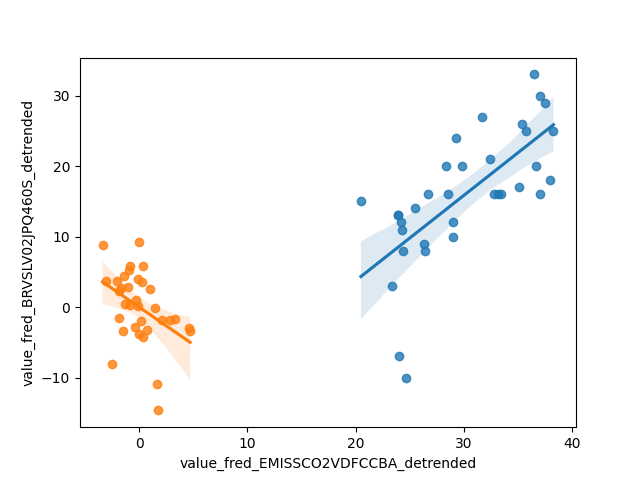
\includegraphics[scale = 0.9]{plots/plot_2026-09-16_detrended.png}
\caption{Detrended Regression Plot for 2026-09-16}
\end{figure}
\newpage
